\section{An abstract machine for switches}
\label{s:absmachine}

\begin{figure*}[!t]
  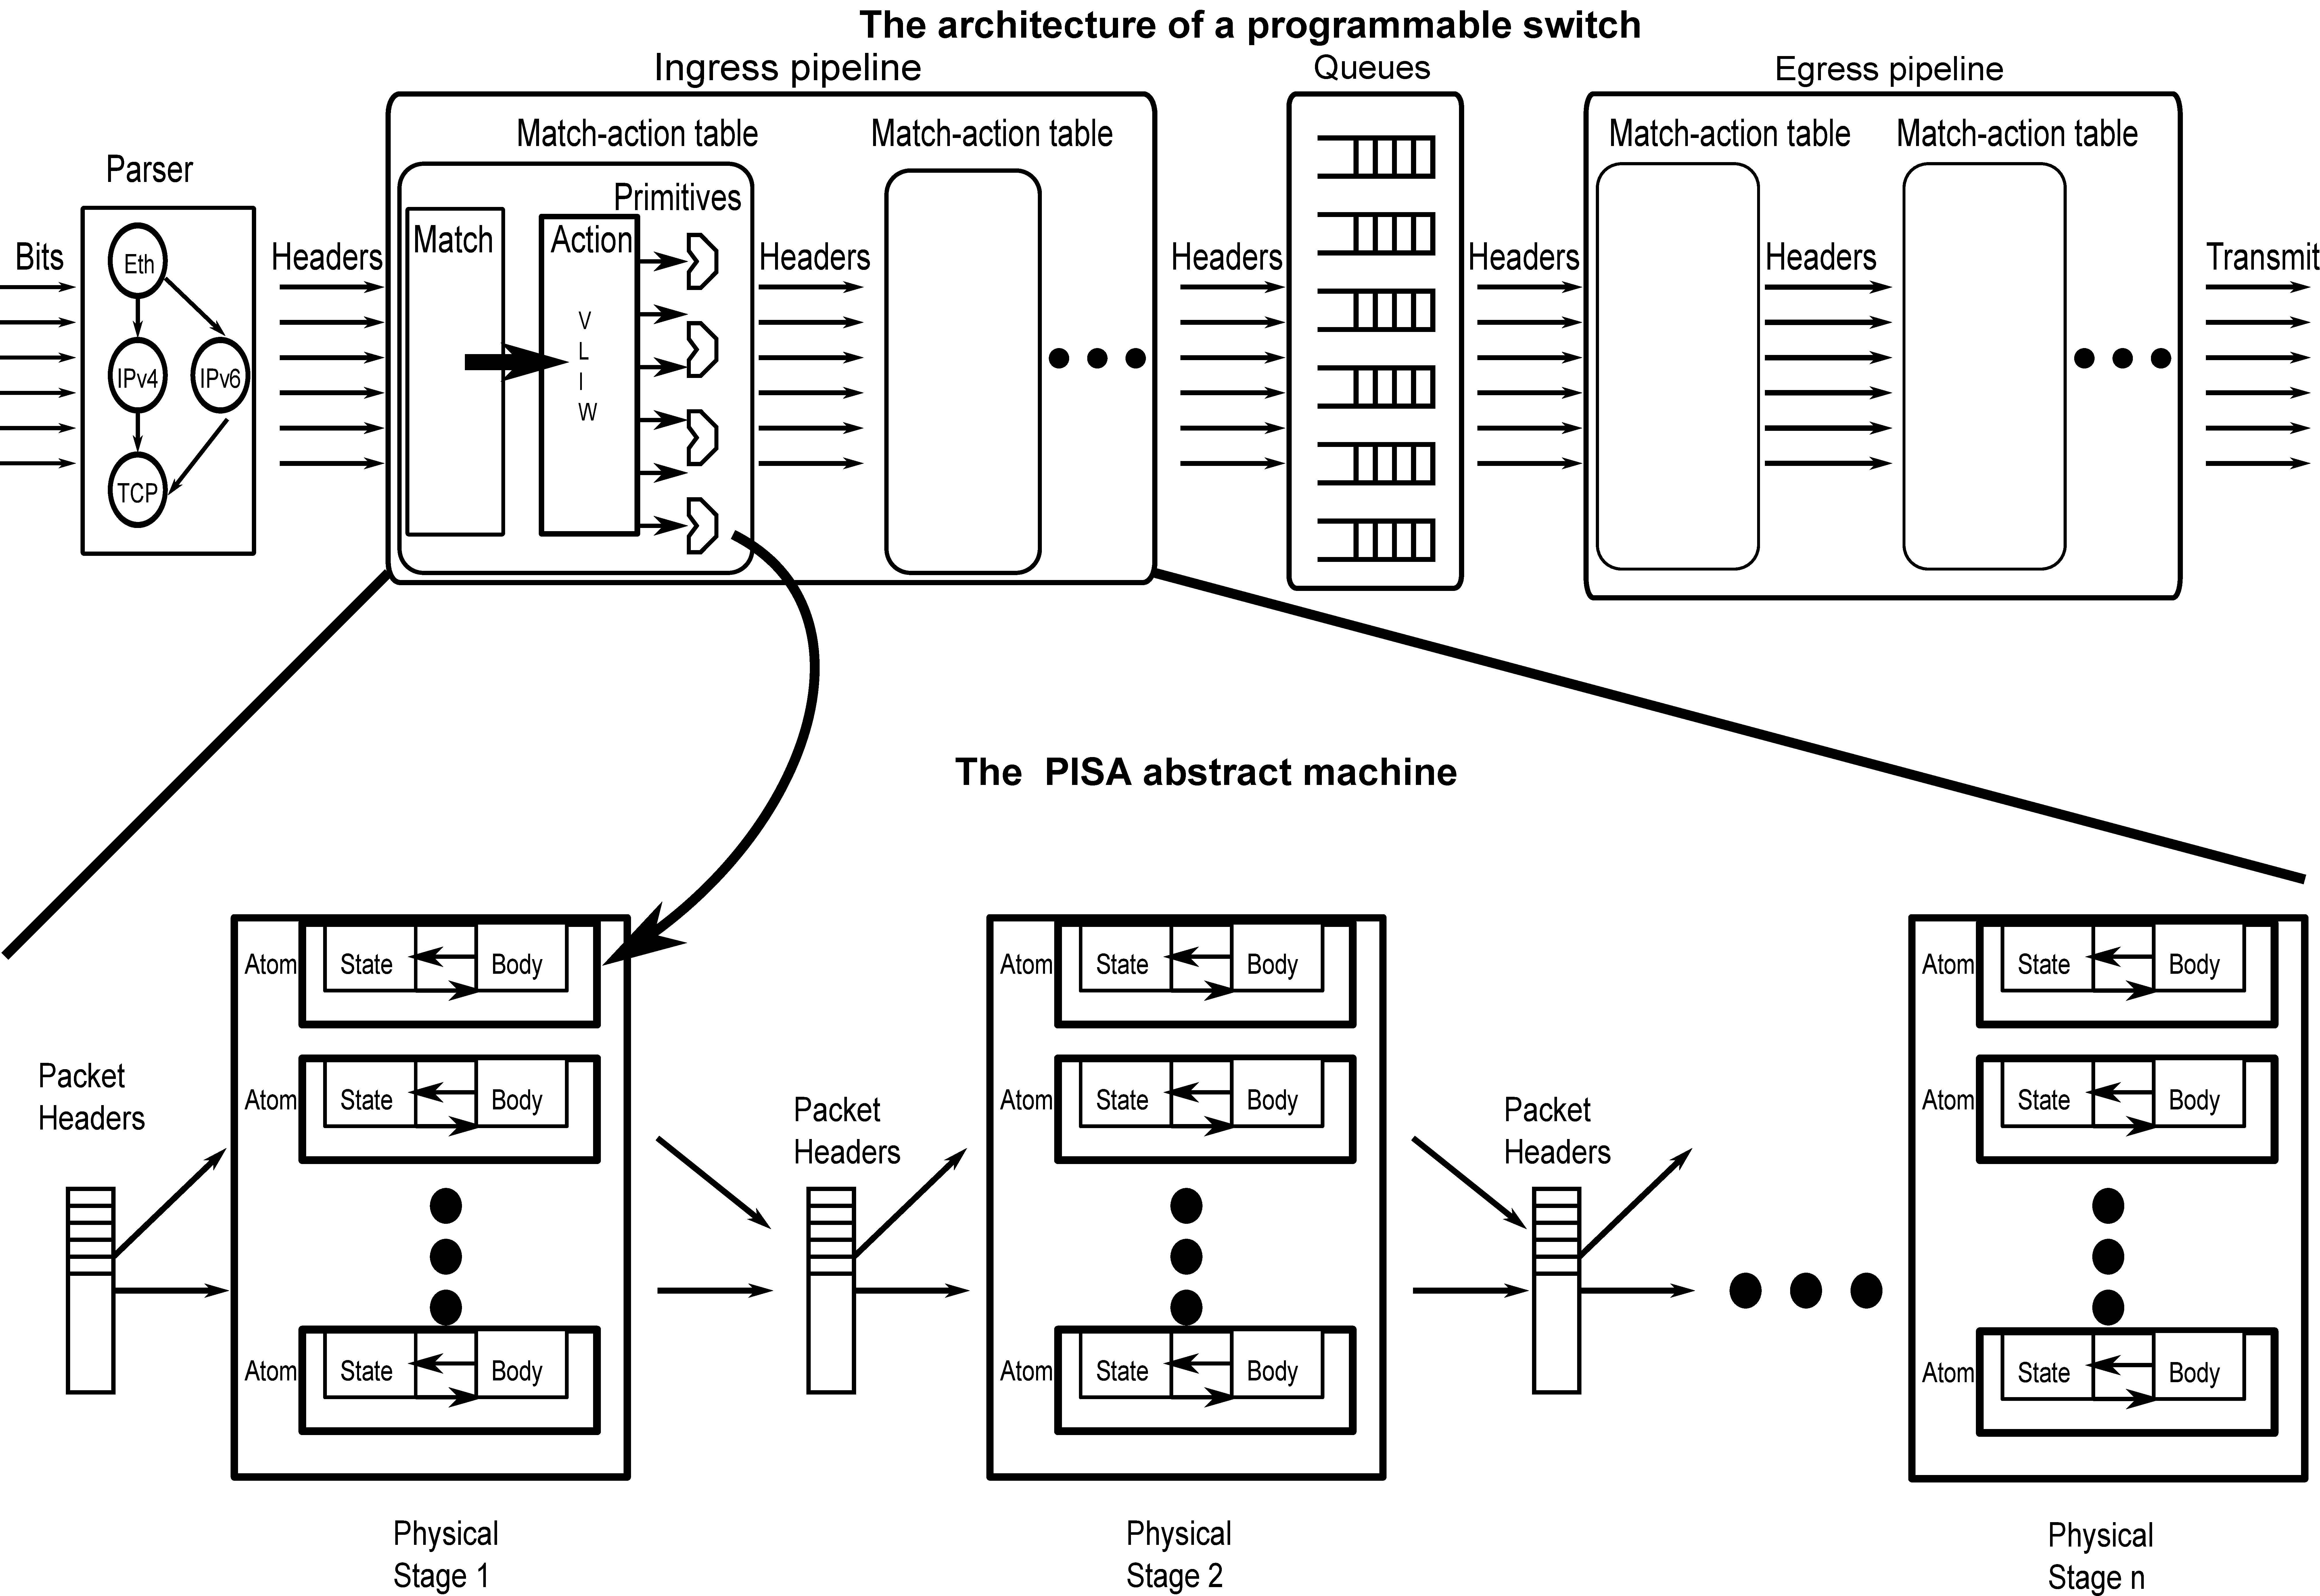
\includegraphics[width=\textwidth]{pisa.pdf}
  \caption{The \absmachine abstract machine and its relationship to
  programmable switch architectures.}
  \label{fig:switch}
\end{figure*}

We first describe \absmachine, a family of abstract machines that serve as
compiler targets for \pktlanguage. PISA stands for Protocol-Independent Switch
Architecture and was first mentioned in a workshop talk~\cite{nick_p4}. Here,
we go further, by describing an executable machine model that serve as a family
of compiler targets for \pktlanguage.

\absmachine is inspired by recent programmable switch architectures with
line-rate performance, such as the RMT architecture~\cite{rmt}, Intel's
FlexPipe~\cite{flexpipe} architecture, and Cavium's XPliant Packet
architecture~\cite{xpliant}. These architectures assume the switch model at the
top of Figure~\ref{fig:switch}.

Packets arriving to the switch are parsed by a programmable parser that turns
packets into header fields. These header fields are first processed by an
ingress pipeline consisting of match-action tables arranged in stages.
Following the ingress pipeline, the packet is queued. Once the packet is
dequeued by the switch scheduler, it is processed by a similar egress pipeline
before being transmitted from the switch.

\absmachine models a switch pipeline such as the ingress or egress pipeline. A
pipeline consists of a number of pipeline stages that execute synchronously on
every time step. Each stage has one time step of latency; the inverse of this
time step is the line rate supported by the pipeline. Once a pipeline stage
processes a packet, it hands it off to the next pipeline stage.

As an abstract machine, \absmachine only models components critical to
data-plane algorithms. In particular, it models the computation that happens in
a match-action table in a stage (i.e. the action half of the match-action
table), but not the match semantics (e.g., direct, ternary, or longest prefix).
\absmachine also does not model packet parsing and assumes that packets
arriving to it are already parsed.

\subsection{Atoms: \absmachine's processing units}

Each pipeline stage contains a vector of \textit{atoms}, with the atoms
executing in parallel. Informally, an atom is an atomic unit of packet
processing provided natively by a \absmachine machine and is represented as a
sequential code block. An atom completes execution and modifies a packet before
the next packet is processed by that atom.

An atom may also contain internal state that persists across packets and
influences the atom's behavior from one packet to the next. For instance, a
switch counter could be written as an atom as follows.\footnote{We use
  p.x to represent field x within a packet p and x to represent
  the state variable x that persists across packets.}
  \begin{lstlisting}[style=customc]
  p.tmp     = counter;
  p.tmp2    = p.tmp + 1;
  counter   = p.tmp2;
  \end{lstlisting}
Similarly, a stateless operation that sets a packet field (such as P4's
modify\_field primitive~\cite{p4spec}) can be written as the atom
below:
\begin{lstlisting}[style=customc]
p.field   = value;
\end{lstlisting}

\absmachine generalizes several aspects of existing programmable switch
architectures. The vector of atoms in each stage generalizes RMT's very-large
instruction-word (VLIW)~\cite{rmt} that executes primitive actions on packet
fields in parallel. Internal state within an atom models persistent switch
state such as meters, counters, and P4's register abstraction in a unified
manner. We assume all state is initialized by the switch control plane, which
we don't explicitly model in \absmachine.

\subsection{Constraining atoms}
\absmachine assumes a synchronous pipeline where each atom executes on every
time step, reading packet fields at the beginning and writing packet fields at
the end of the time step. All writes happen simultaneously at the end
of a time step; so, \absmachine forbids two atoms in a stage from writing to
the same packet field to remove all data races.

To provide deterministic performance at line rate, atoms must be suitably
constrained.  We impose two such constraints that distinguish \absmachine from
software routers~\cite{click} and network processors~\cite{ixp4xx} that
sacrifice determinism for programmability.

First, \absmachine machines are \textit{shared-nothing}: state variables are
internal to an atom. Their values can only be communicated to atoms in
subsequent stages by writing them into packet fields. This restriction reflects
the capabilities of line-rate switches: accessing shared memory from multiple
switch stages is technically challenging because it requires multi-ported RAMs
and routing long wires on the chip.

Second, we constrain the complexity of atoms by defining {\it atom templates}
(\S\ref{ss:code_gen}).  Informally, an atom template is a program that is
guaranteed to terminate and specifies how atoms are executed. One example is an
ALU with a restricted set of primitive operations to choose from
(Figure~\ref{fig:alu_in_sketch}). Atom templates allow us to create different
\absmachine machines that support different atoms natively. As programmable
switches evolve, we expect the computational capabilities of atoms to evolve as
well. However, atoms cannot be arbitrarily complex: a programmable switch's
line rate is inversely proportional to the maximum execution latency of all its
atoms.
